\documentclass[11pt]{article}
\usepackage[textwidth=18.0cm, textheight=23.0cm, top=2.0cm]{geometry}
\usepackage{pst-all}
\usepackage{amssymb}
\usepackage{tikz}
\usepackage{underscore}\begin{document}
\pagestyle{empty}


ClassName: \underline{\textbf{Class_10.2bp-9}}
\par
BinSize: \underline{\textbf{100 × 100}}
\par
ReduceSize: \underline{\textbf{100 × 100}}
\par
TypeNum: \underline{\textbf{20}}
\par
Num: \underline{\textbf{20}}
\par
OutS: \underline{\textbf{30000}}
\par
InS: \underline{\textbf{19646}}
\par
Rate: \underline{\textbf{0.655}}
\par
UB: \underline{\textbf{3}}
\par
LB0: \underline{\textbf{3}}
\par
LB: \underline{\textbf{3}}
\par
LBWithCut: \underline{\textbf{3}}
\par
NodeCut: \underline{\textbf{0}}
\par
ExtendedNodeCnt: \underline{\textbf{1}}
\par
GenNodeCnt: \underline{\textbf{1}}
\par
PrimalNode: \underline{\textbf{0}}
\par
ColumnCount: \underline{\textbf{3}}
\par
TotalCutCount: \underline{\textbf{0}}
\par
RootCutCount: \underline{\textbf{0}}
\par
LPSolverCnt: \underline{\textbf{1}}
\par
PricingSolverCnt: \underline{\textbf{0}}
\par
BranchAndBoundNum: \underline{\textbf{1}}
\par
isOpt: \underline{\textbf{true}}
\par
TimeOnInitSolution: \underline{\textbf{600.000 s}}
\par
TimeOnPrimal: \underline{\textbf{0.000 s}}
\par
TimeOnPricing: \underline{\textbf{0.000 s}}
\par
TimeOnRmp: \underline{\textbf{0.060 s}}
\par
TotalTime: \underline{\textbf{600.323 s}}
\par
\newpage


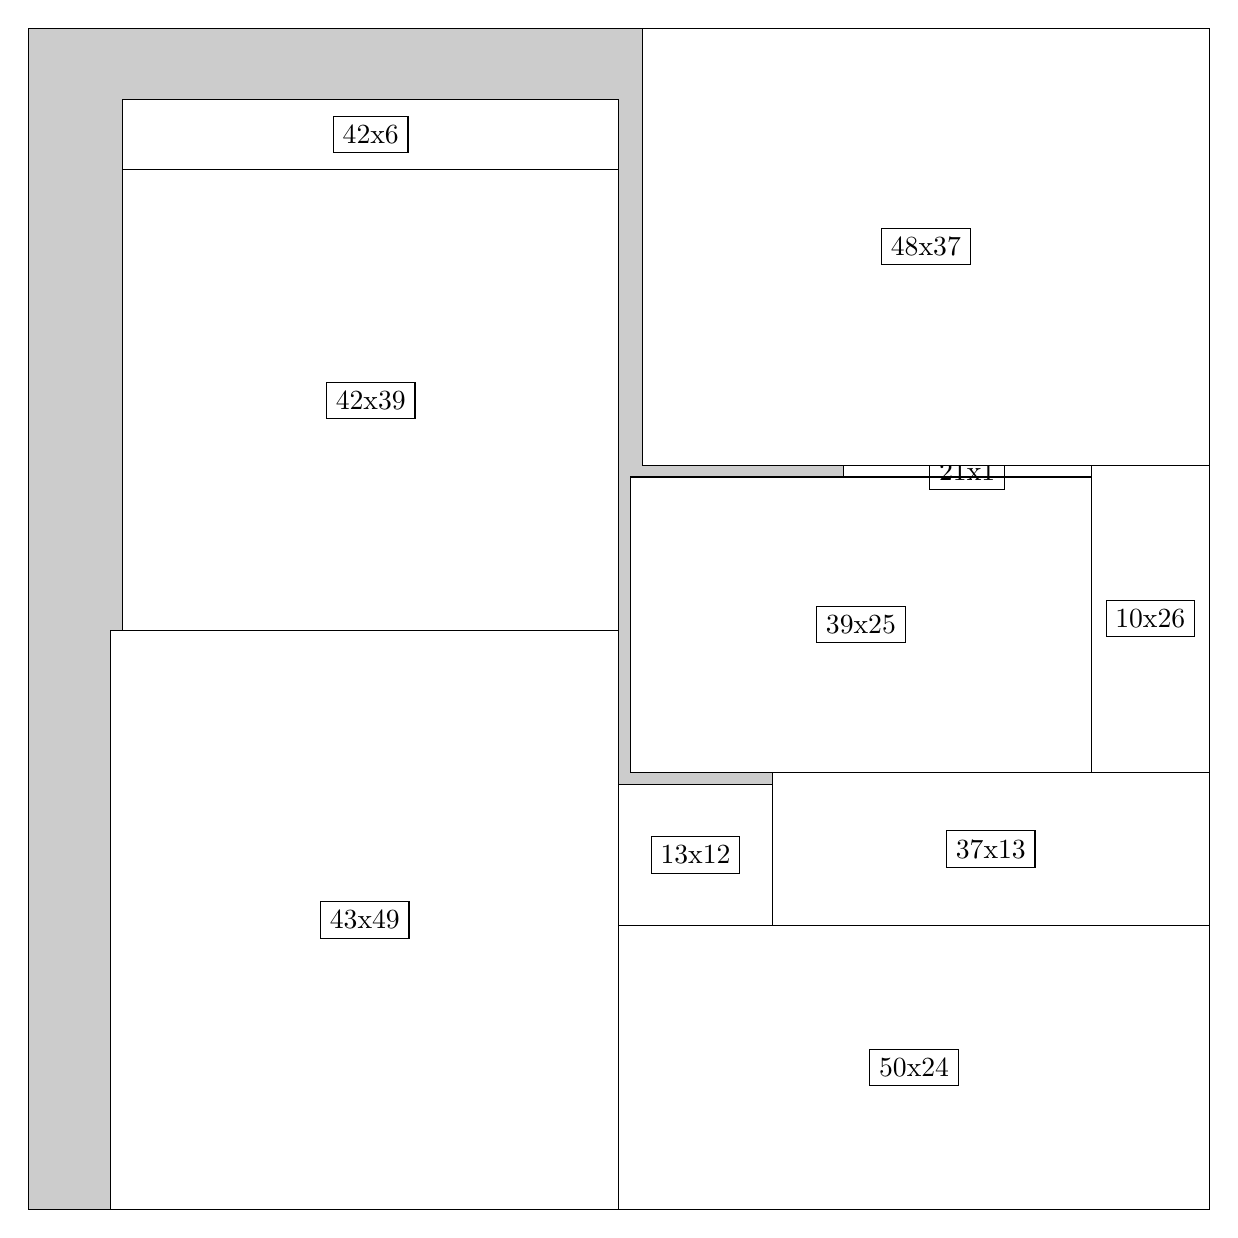
\begin{tikzpicture}[shorten >=1pt,scale=1.0,every node/.style={scale=1.0},->]
\tikzstyle{vertex}=[circle,fill=black!25,minimum size=14pt,inner sep=0pt]
\filldraw[fill=gray!40!white, draw=black] (0,0) rectangle (15.0,15.0);
\foreach \name/\x/\y/\w/\h in {50x24/7.5/0.0/7.5/3.5999999999999996,37x13/9.45/3.5999999999999996/5.55/1.95,13x12/7.5/3.5999999999999996/1.95/1.7999999999999998,10x26/13.5/5.55/1.5/3.9,39x25/7.6499999999999995/5.55/5.85/3.75,21x1/10.35/9.299999999999999/3.15/0.15,48x37/7.8/9.45/7.199999999999999/5.55,43x49/1.05/0.0/6.45/7.35,42x39/1.2/7.35/6.3/5.85,42x6/1.2/13.2/6.3/0.8999999999999999}
\filldraw[fill=white!40!white, draw=black] (\x,\y) rectangle node[draw] (\name) {\name} ++(\w,\h);
\end{tikzpicture}


w =50 , h =24 , x =50 , y =0 , v =1200
\par
w =37 , h =13 , x =63 , y =24 , v =481
\par
w =13 , h =12 , x =50 , y =24 , v =156
\par
w =10 , h =26 , x =90 , y =37 , v =260
\par
w =39 , h =25 , x =51 , y =37 , v =975
\par
w =21 , h =1 , x =69 , y =62 , v =21
\par
w =48 , h =37 , x =52 , y =63 , v =1776
\par
w =43 , h =49 , x =7 , y =0 , v =2107
\par
w =42 , h =39 , x =8 , y =49 , v =1638
\par
w =42 , h =6 , x =8 , y =88 , v =252
\par
\newpage


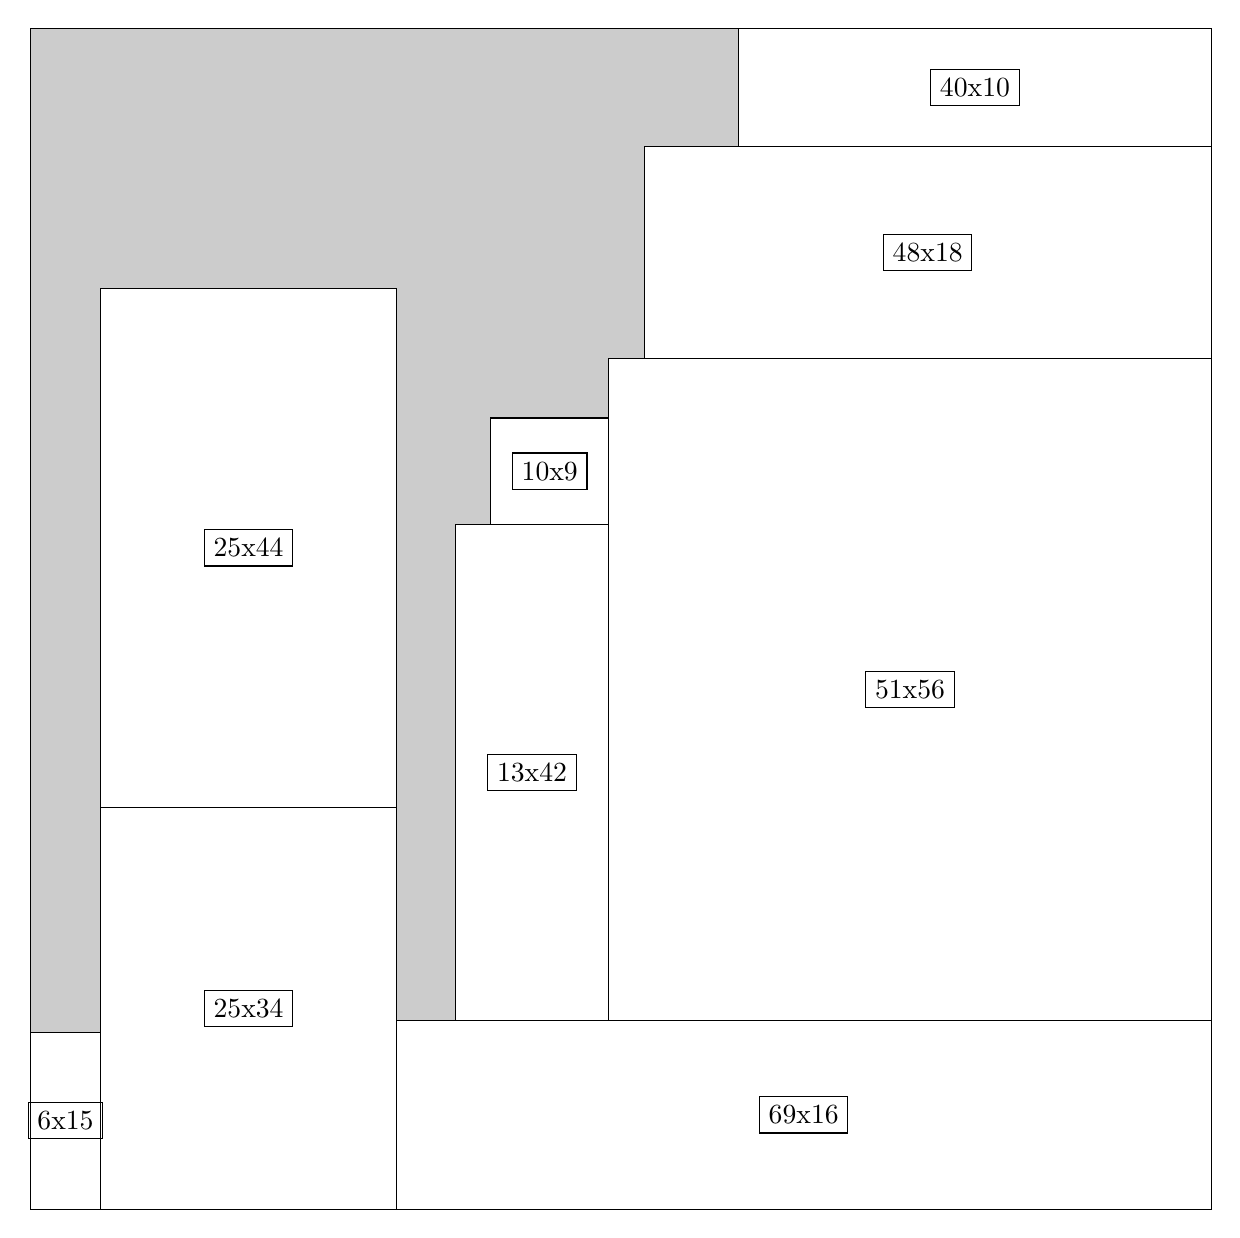
\begin{tikzpicture}[shorten >=1pt,scale=1.0,every node/.style={scale=1.0},->]
\tikzstyle{vertex}=[circle,fill=black!25,minimum size=14pt,inner sep=0pt]
\filldraw[fill=gray!40!white, draw=black] (0,0) rectangle (15.0,15.0);
\foreach \name/\x/\y/\w/\h in {69x16/4.6499999999999995/0.0/10.35/2.4,51x56/7.35/2.4/7.6499999999999995/8.4,13x42/5.3999999999999995/2.4/1.95/6.3,10x9/5.85/8.7/1.5/1.3499999999999999,48x18/7.8/10.799999999999999/7.199999999999999/2.6999999999999997,40x10/9.0/13.5/6.0/1.5,25x34/0.8999999999999999/0.0/3.75/5.1,6x15/0.0/0.0/0.8999999999999999/2.25,25x44/0.8999999999999999/5.1/3.75/6.6}
\filldraw[fill=white!40!white, draw=black] (\x,\y) rectangle node[draw] (\name) {\name} ++(\w,\h);
\end{tikzpicture}


w =69 , h =16 , x =31 , y =0 , v =1104
\par
w =51 , h =56 , x =49 , y =16 , v =2856
\par
w =13 , h =42 , x =36 , y =16 , v =546
\par
w =10 , h =9 , x =39 , y =58 , v =90
\par
w =48 , h =18 , x =52 , y =72 , v =864
\par
w =40 , h =10 , x =60 , y =90 , v =400
\par
w =25 , h =34 , x =6 , y =0 , v =850
\par
w =6 , h =15 , x =0 , y =0 , v =90
\par
w =25 , h =44 , x =6 , y =34 , v =1100
\par
\newpage



\begin{tikzpicture}[shorten >=1pt,scale=1.0,every node/.style={scale=1.0},->]
\tikzstyle{vertex}=[circle,fill=black!25,minimum size=14pt,inner sep=0pt]
\filldraw[fill=gray!40!white, draw=black] (0,0) rectangle (15.0,15.0);
\foreach \name/\x/\y/\w/\h in {80x36/3.0/0.0/12.0/5.3999999999999995}
\filldraw[fill=white!40!white, draw=black] (\x,\y) rectangle node[draw] (\name) {\name} ++(\w,\h);
\end{tikzpicture}


w =80 , h =36 , x =20 , y =0 , v =2880
\par
\newpage


\end{document}